\documentclass[review]{elsarticle}
%-----------------------------------------------------

\usepackage{amsmath}
\usepackage{graphicx}

\graphicspath{{./figs/}}

\newcommand{\ihat}{\boldsymbol{\hat{\textbf{\i}}}}
\newcommand{\jhat}{\boldsymbol{\hat{\textbf{\j}}}}
\newcommand{\roughly}{{\raise.17ex\hbox{$\scriptstyle\sim$}}}
\newcommand{\dmax}{d_\text{max}}
\newcommand{\dmin}{d_\text{min}}

%-----------------------------------------------------

\makeatletter
\renewcommand{\fnum@figure}{Figure 9}
\makeatother

\thispagestyle{empty}

\begin{document}
\allowdisplaybreaks

\begin{figure}[ht]
\centering
%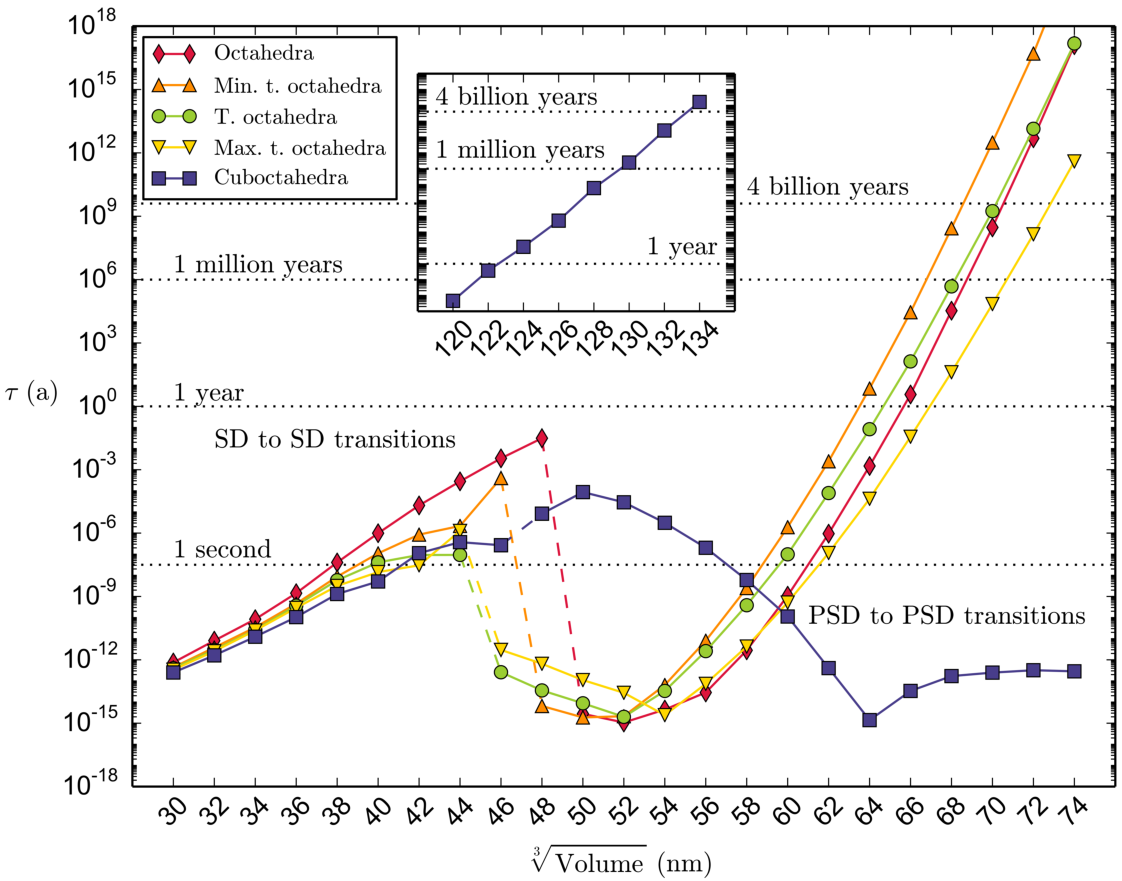
\includegraphics[width=\textwidth]{Figure_09_HR.pdf}
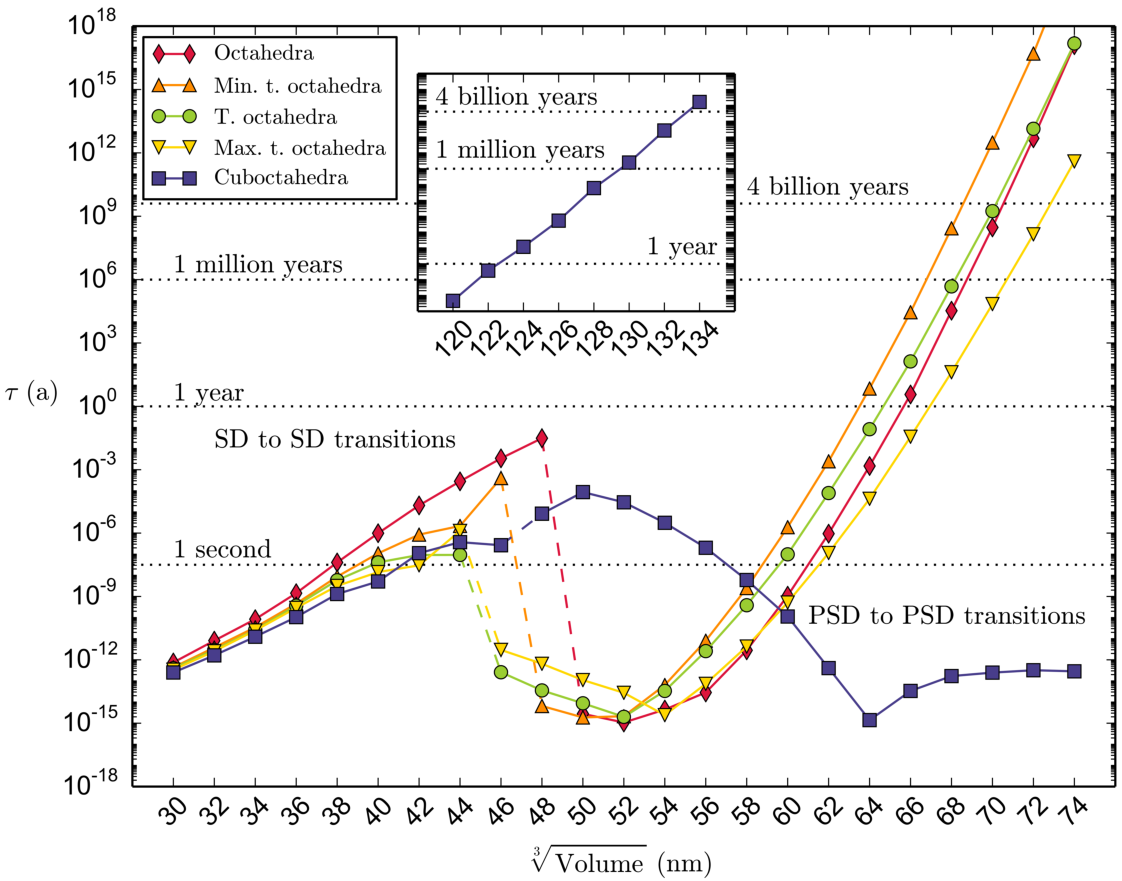
\includegraphics[width=\textwidth]{Figure_09.pdf}
\caption{Relaxation times for the euhedral shapes. The relaxation times are calculated with $\tau_0=1\,\text{ns}$, $T=300\,\text{K}$. $\tau$ increases exponentially for the SD--SD transitions, but reaches only laboratory scale stabilities before the SD--PSD threshold. The (truncated) octahedral shapes show a dip in the stability in the lower end of the PSD range for HAV--HAV and IAV--IAV transitions, reaching a minimum at $\roughly$52$\,\text{nm}$. Once the EAVs have the lowest energies, the relaxation times grow exponentially with size, reaching four billion years from $\roughly$70$\,\text{nm}$. The cuboctahedra, however, show a different behaviour: they do not show a dip in the stability for the first HAV--HAV transitions, but with increasing size they produce lower relaxation times as the energy of the dIAV gets closer. The relaxation times for the transitions between dIAVs plateau up to 74$\,\text{nm}$. Exponential growth of the relaxation times occurs from $\roughly$110$\,\text{nm}$ (inset), surpassing four billion years from $\roughly$134$\,\text{nm}$.}
\label{fig9}
\end{figure}

\end{document}